% This is text associated with the open textbook "Open Electromagnetics"
% See immediately below for author, date
% This work is licensed under the Creative Commons Attribution-ShareAlike 4.0 International License. (CC BY SA 4.0) 
% To view a copy of the license, visit http://creativecommons.org/licenses/by-sa/4.0/

%ORB TITLE Uniform Plane Waves: Derivation
%ORB AUTHOR 0        # S.W. Ellingson, Virginia Tech (ellingson@vt.edu)
%ORB DATE 20180807   # yyyymmdd
%ORB ABSTRACT Uniform Plane Waves: Derivation

\label{m0038_Uniform_Plane_Waves_Derivation} % <-- Must match name of this file and module directory name.  Don't mess with this!
\index{waves!plane|(}

Section~\ref{m0036_Wave_Equations_SourceFree_Lossless} showed how Maxwell's Equations could be reduced to a pair of phasor-domain ``wave equations,'' namely:
%
\begin{equation}
\nabla^2\widetilde{\bf E} +\beta^2 \widetilde{\bf E} = 0 
\label{m0038_eWEE2}
\end{equation}
%
\begin{equation}
\nabla^2\widetilde{\bf H} +\beta^2 \widetilde{\bf H} = 0 
\label{m0038_eWEH2}
\end{equation}
%
where $\beta=\omega\sqrt{\mu\epsilon}$, assuming unbounded homogeneous, isotropic, lossless, and source-free media.
In this section, we solve these equations for the special case of a uniform plane wave.
A uniform plane wave is one for which both $\widetilde{\bf E}$ and $\widetilde{\bf H}$ have constant magnitude and phase in a specified plane.  
Despite being a special case, the solution turns out to be broadly applicable, appearing as a common building block in many practical and theoretical problems in unguided propagation (as explained in Section~\ref{m0142_Types_of_Waves}), as well as in more than a few transmission line and waveguide problems.

To begin, let us assume that the plane over which $\widetilde{\bf E}$ and $\widetilde{\bf H}$ have constant magnitude and phase is a plane of constant $z$. 
% We will work the problem using the Cartesian coordinate system.
First, note that we may make this assumption with no loss of generality.
For example, we could alternatively select a plane of constant $y$, solve the problem, and then simply exchange variables to get a solution for planes of constant $z$ (or $x$).\footnote{By the way, this is a highly-recommended exercise for the student.}
%%% TODO Above
Furthermore, the solution for any planar orientation not corresponding to a plane of constant $x$, $y$, or $z$ may be similarly obtained by a rotation of coordinates, since the physics of the problem does not depend on the orientation of this plane -- if it does, then the medium is not isotropic!
 
We may express the constraint that the magnitude and phase of $\widetilde{\bf E}$ and $\widetilde{\bf H}$ are constant over a plane that is perpendicular to the $z$ axis as follows:
%
\begin{equation}
\frac{\partial}{\partial x} \widetilde{\bf E} = \frac{\partial}{\partial y} \widetilde{\bf E} 
= \frac{\partial}{\partial x} \widetilde{\bf H} = \frac{\partial}{\partial y} \widetilde{\bf H} 
= 0
\label{m0038_eWEPWP}
\end{equation}
%
Let us identify the Cartesian components of each of these fields as follows: 
%
\begin{flalign}
\widetilde{\bf E} &= \hat{\bf x}\widetilde{E}_x+\hat{\bf y}\widetilde{E}_y+\hat{\bf z}\widetilde{E}_z ~\mbox{, and} \\
\widetilde{\bf H} &= \hat{\bf x}\widetilde{H}_x+\hat{\bf y}\widetilde{H}_y+\hat{\bf z}\widetilde{H}_z
\end{flalign}
%
Now Equation~\ref{m0038_eWEPWP} may be interpreted in detail for $\widetilde{\bf E}$ as follows:
%
\begin{flalign}
\frac{\partial}{\partial x} \widetilde{E}_x = \frac{\partial}{\partial x} \widetilde{E}_y = \frac{\partial}{\partial x} \widetilde{E}_z &= 0 \label{m0038_eECxC} \\
\frac{\partial}{\partial y} \widetilde{E}_x = \frac{\partial}{\partial y} \widetilde{E}_y = \frac{\partial}{\partial y} \widetilde{E}_z &= 0 \label{m0038_eECyC}
\end{flalign}
%
and for $\widetilde{\bf H}$ as follows:
%
\begin{flalign}
\frac{\partial}{\partial x} \widetilde{H}_x = \frac{\partial}{\partial x} \widetilde{H}_y = \frac{\partial}{\partial x} \widetilde{H}_z &= 0 \\
\frac{\partial}{\partial y} \widetilde{H}_x = \frac{\partial}{\partial y} \widetilde{H}_y = \frac{\partial}{\partial y} \widetilde{H}_z &= 0 
\end{flalign}

The wave equation for $\widetilde{\bf E}$ (Equation~\ref{m0038_eWEE2}) written explicitly in Cartesian coordinates is
%
\begin{flalign}
\left[ \frac{\partial^2}{\partial x^2}  
+ \frac{\partial^2}{\partial y^2}  
+ \frac{\partial^2}{\partial z^2} \right]
&\left( \hat{\bf x}\widetilde{E}_x+\hat{\bf y}\widetilde{E}_y+\hat{\bf z}\widetilde{E}_z \right) \nonumber \\
+\beta^2 
&\left( \hat{\bf x}\widetilde{E}_x+\hat{\bf y}\widetilde{E}_y+\hat{\bf z}\widetilde{E}_z \right)
 = 0 
\end{flalign}
%  
Decomposing this equation into separate equations for each of the three coordinates, we obtain the following:
%
\begin{equation}
\left[ \frac{\partial^2}{\partial x^2} + \frac{\partial^2}{\partial y^2} + \frac{\partial^2}{\partial z^2} \right] \widetilde{E}_x + \beta^2 \widetilde{E}_x = 0 
\label{m0038_eECx}
\end{equation}
%
\begin{equation}
\left[ \frac{\partial^2}{\partial x^2} + \frac{\partial^2}{\partial y^2} + \frac{\partial^2}{\partial z^2} \right] \widetilde{E}_y + \beta^2 \widetilde{E}_y = 0 
\label{m0038_eECy}
\end{equation}
%
\begin{equation}
\left[ \frac{\partial^2}{\partial x^2} + \frac{\partial^2}{\partial y^2} + \frac{\partial^2}{\partial z^2} \right] \widetilde{E}_z + \beta^2 \widetilde{E}_z = 0 
\label{m0038_eECz}
\end{equation}
%%
Applying the constraints of Equations~\ref{m0038_eECxC} and \ref{m0038_eECyC}, we note that many of the terms in Equations~\ref{m0038_eECx}--\ref{m0038_eECz} are zero.  We are left with:
%
\begin{flalign}
\frac{\partial^2}{\partial z^2} \widetilde{E}_x + \beta^2 \widetilde{E}_x &= 0 \label{m0038_eWEPWE1} \\
\frac{\partial^2}{\partial z^2} \widetilde{E}_y + \beta^2 \widetilde{E}_y &= 0 \label{m0038_eWEPWE2} \\
\frac{\partial^2}{\partial z^2} \widetilde{E}_z + \beta^2 \widetilde{E}_z &= 0 \label{m0038_eWEPWE3}
%
\end{flalign}

Now we will show that Equation~\ref{m0038_eWEPWP} also implies that $\widetilde{E}_z$ must be zero.  
To show this, we use Ampere's Law for a source-free region (Section~\ref{m0036_Wave_Equations_SourceFree_Lossless}):
%
\begin{equation}
\nabla \times \widetilde{\bf H} = +j\omega\epsilon\widetilde{\bf E}
\end{equation}
%
and take the dot product with $\hat{\bf z}$ on both sides:
%
\begin{flalign}
\hat{\bf z} \cdot \left( \nabla \times \widetilde{\bf H} \right) &= +j\omega\epsilon \widetilde{E}_z \nonumber \\
\frac{\partial}{\partial y}\widetilde{H}_x - \frac{\partial}{\partial x}\widetilde{H}_y  &= +j\omega\epsilon \widetilde{E}_z
\label{m0038_eHxHyEz}
\end{flalign}
%
Again applying the constraints of Equation~\ref{m0038_eWEPWP}, the left side of Equation~\ref{m0038_eHxHyEz} must be zero; therefore, $\widetilde{E}_z=0$.  
The exact same procedure applied to $\widetilde{\bf H}$ (using the Maxwell-Faraday Equation; also given in Section~\ref{m0036_Wave_Equations_SourceFree_Lossless}) reveals that $\widetilde{H}_z$ is also zero.\footnote{Showing this is a highly-recommended exercise for the reader.} 
%%% TODO Above
Here is what we have found:
%
%ORB HIGHLIGHT
\begin{mdframed}[backgroundcolor=yellow!20,nobreak=true] 
If a wave is uniform over a plane, then the electric and magnetic field vectors must lie in this plane.
\end{mdframed}
%
This conclusion is a direct consequence of the fact that Maxwell's Equations require the electric field to be proportional to the curl of the magnetic field and vice-versa.  

The general solution to Equation~\ref{m0038_eWEPWE1} is:   
%
\begin{equation}
\widetilde{E}_x = E_{x0}^+ e^{-j\beta z} + E_{x0}^- e^{+j\beta z}
\label{m0038_ePWLM-Ex} 
\end{equation}
%
where $E_{x0}^+$ and $E_{x0}^-$ are complex-valued constants.  
The values of these constants are determined by boundary conditions -- possibly sources -- outside the region of interest.
Since in this section we are limiting our scope to source-free and homogeneous regions, we may for the moment consider the values of $E_{x0}^+$ and $E_{x0}^-$ to be arbitrary, since any values will satisfy the associated wave equation.\footnote{The reader is encouraged to confirm that these are solutions by substitution into the associated wave equation.}
%%% TODO Above

Similarly we have for $\widetilde{E}_y$:
%
\begin{equation}
\widetilde{E}_y = E_{y0}^+ e^{-j\beta z} + E_{y0}^- e^{+j\beta z}
\label{m0038_ePWLM-Ey} 
\end{equation}
%
where $E_{y0}^+$ and $E_{y0}^-$ are again arbitrary constants.  
Summarizing, we have found
%
\begin{equation}
\widetilde{\bf E} = \hat{\bf x}\widetilde{E}_x + \hat{\bf y}\widetilde{E}_y 
\end{equation}
%
where $\widetilde{E}_x$ and $\widetilde{E}_y$ are given by Equations~\ref{m0038_ePWLM-Ex} and \ref{m0038_ePWLM-Ey}, respectively.

Note that Equations~\ref{m0038_ePWLM-Ex} and \ref{m0038_ePWLM-Ey} are essentially the \emph{same} equations encountered in the study of waves in lossless transmission lines; for a reminder, see Section~\ref{m0027_Wave_Equations_for_a_Transmission_Line}.  Specifically, factors containing $e^{-j\beta z}$ describe propagation in the $+z$ direction, whereas factors containing $e^{+j\beta z}$ describe propagation in the $-z$ direction.  We conclude:
%
%ORB HIGHLIGHT
\begin{mdframed}[backgroundcolor=yellow!20,nobreak=true] 
If a wave is uniform over a plane, then possible directions of propagation are the two directions perpendicular to the plane. 
\end{mdframed}
%
Since we previously established that the electric and magnetic field vectors must lie in the plane, we also conclude:
%
%ORB HIGHLIGHT
\begin{mdframed}[backgroundcolor=yellow!20,nobreak=true] 
The direction of propagation is perpendicular to the electric and magnetic field vectors.
\end{mdframed}
%
This conclusion turns out to be generally true; i.e., it is not limited to uniform plane waves.  
Although we will not provide a rigorous proof of this, one way to see that this is true is to imagine that any type of wave can be interpreted as the sum (formally, a \emph{linear combination}) of uniform plane waves, so perpendicular orientation of the field vectors with respect to the direction of propagation is inescapable.  

The same procedure yields the uniform plane wave solution to the wave equation for $\widetilde{\bf H}$, which is
%
\begin{equation}
\widetilde{\bf H} = \hat{\bf x}\widetilde{H}_x + \hat{\bf y}\widetilde{H}_y 
\end{equation}
%
where
%
\begin{equation}
\widetilde{H}_x = H_{x0}^+ e^{-j\beta z} + H_{x0}^- e^{+j\beta z}
\label{m0038_ePWLM-Hx} 
\end{equation}
%
\begin{equation}
\widetilde{H}_y = H_{y0}^+ e^{-j\beta z} + H_{y0}^- e^{+j\beta z}
\label{m0038_ePWLM-Hy} 
\end{equation}
%
and where $H_{x0}^+$, $H_{x0}^-$, $H_{y0}^+$ and $H_{y0}^-$ are arbitrary constants.
Note that the solution is essentially the same as that for $\widetilde{\bf E}$, with the sole difference being that the arbitrary constants may apparently have different values. 

To this point, we have seen no particular relationship between the electric and magnetic fields, and it may appear that the electric and magnetic fields are independent of each other.
However, Maxwell's Equations -- specifically, the two curl equations -- make it clear that there must be a relationship between these fields.
Subsequently the arbitrary constants in the solutions for $\widetilde{\bf E}$ and $\widetilde{\bf H}$ must also be related.
In fact, there are two considerations here:
%
\begin{itemize}
\item The \emph{magnitude and phase} of $\widetilde{\bf E}$ must be related to the magnitude and phase of $\widetilde{\bf H}$.  
Since both fields are solutions to the same differential (wave) equation, they may differ by no more than a multiplicative constant.
Since the units of $\widetilde{\bf E}$ and $\widetilde{\bf H}$ are V/m and A/m respectively, this constant must be expressible in units of V/m divided by A/m; i.e., in units of $\Omega$, an impedance.
\item The \emph{direction} of $\widetilde{\bf E}$ must be related to direction of $\widetilde{\bf H}$.    
\end{itemize}
%
Let us now address these considerations.
Consider an electric field that points in one of the cardinal directions -- let's say $+\hat{\bf x}$ -- and make the definition $E_0 \triangleq E_{x0}^+$ for notational convenience.
Then the electric field intensity may be written as follows:
%
\begin{equation}
\widetilde{\bf E} = \hat{\bf x}E_0 e^{-j\beta z}
\label{m0038_eEx}
\end{equation}
%
Again, there is no loss of generality here since the coordinate system could be rotated in such a way that \emph{any} uniform plane could be described in this way. 

We may now determine $\widetilde{\bf H}$ from $\widetilde{\bf E}$ using the Maxwell-Faraday Equation 
\index{Maxwell-Faraday equation}
(Section~\ref{m0036_Wave_Equations_SourceFree_Lossless}):
%
\begin{equation}
\nabla \times  \widetilde{\bf E} = -j\omega\mu\widetilde{\bf H}
\end{equation}
%
Solving this equation for $\widetilde{\bf H}$, we find:
%
\begin{equation}
\widetilde{\bf H} = \frac{\nabla \times \widetilde{\bf E} }{-j\omega\mu} 
                  = \frac{\nabla \times \left[ \hat{\bf x}E_0 e^{-j\beta z} \right] }{-j\omega\mu}
\label{m0038_ePWLM-PWRH}
\end{equation}
%
Now let us apply the curl operator.
The complete expression for the curl operator in Cartesian coordinates is given in Section~\ref{m0139_Vector_Operators}.
Here let us consider one component at a time,
starting with the $\hat{\bf x}$ component:
%
\begin{equation}
\hat{\bf x}\cdot
\left( \nabla \times \widetilde{\bf E} \right) = 
\frac{\partial \widetilde{E}_z}{\partial y} - \frac{\partial \widetilde{E}_y}{\partial z} 
\end{equation}
%
Since $\widetilde{E}_y=\widetilde{E}_z=0$, the above expression is zero and subsequently $\widetilde{H}_x=0$.
Next, the $\hat{\bf y}$ component:
%
\begin{equation}
\hat{\bf y}\cdot
\left( \nabla \times \widetilde{\bf E} \right) = 
 \frac{\partial \widetilde{E}_x}{\partial z} - \frac{\partial \widetilde{E}_z}{\partial x} 
\end{equation}
%
Here $\widetilde{E}_z=0$, so we have simply
%
\begin{equation}
%\widetilde{H}_y = 
\hat{\bf y}\cdot
\left( \nabla \times \widetilde{\bf E} \right) = \frac{ \partial \widetilde{E}_x}{\partial z}
\end{equation}
%
It is not necessary to repeat this procedure for $\widetilde{H}_z$, since we know in advance that $\widetilde{\bf H}$ must be perpendicular to the direction of propagation and subsequently $\widetilde{H}_z=0$.
Returning to Equation~\ref{m0038_ePWLM-PWRH}, we obtain:
%
\begin{flalign}
\widetilde{\bf H} &= \hat{\bf y} \frac{ 1 }{-j\omega\mu} \frac{ \partial }{\partial z} \widetilde{E}_x \nonumber \\
                  &= \hat{\bf y} \frac{ 1 }{-j\omega\mu} \frac{ \partial}{\partial z} \left( E_0 e^{-j\beta z} \right) \nonumber \\
                  &= \hat{\bf y} \frac{ 1 }{-j\omega\mu} \left( -j\beta E_0 e^{-j\beta z} \right) \nonumber \\
                  &= \hat{\bf y} \frac{ \beta }{\omega\mu} E_0 e^{-j\beta z} 
\label{m0038_eHy}
\end{flalign}

Note that $\widetilde{\bf H}$ points in the $+\hat{\bf y}$ direction.
So, as expected, both $\widetilde{\bf E}$ and $\widetilde{\bf H}$ are perpendicular to the direction of propagation.
However, we have now found a more specific relationship: $\widetilde{\bf E}$ and $\widetilde{\bf H}$ are perpendicular \emph{to each other}.
Just as $\hat{\bf x} \times \hat{\bf y} = \hat{\bf z}$, we see that $\widetilde{\bf E} \times \widetilde{\bf H}$ points in the direction of propagation.
This is illustrated in Figure~\ref{m0038_fEHk}.
Summarizing:
%
%ORB HIGHLIGHT
\begin{mdframed}[backgroundcolor=yellow!20,nobreak=true] 
$\widetilde{\bf E}$, $\widetilde{\bf H}$, and the direction of propagation $\widetilde{\bf E} \times \widetilde{\bf H}$ are mutually perpendicular.
\end{mdframed}
%
\begin{figure}
\begin{center}
\pdftooltip{{  % note double braces
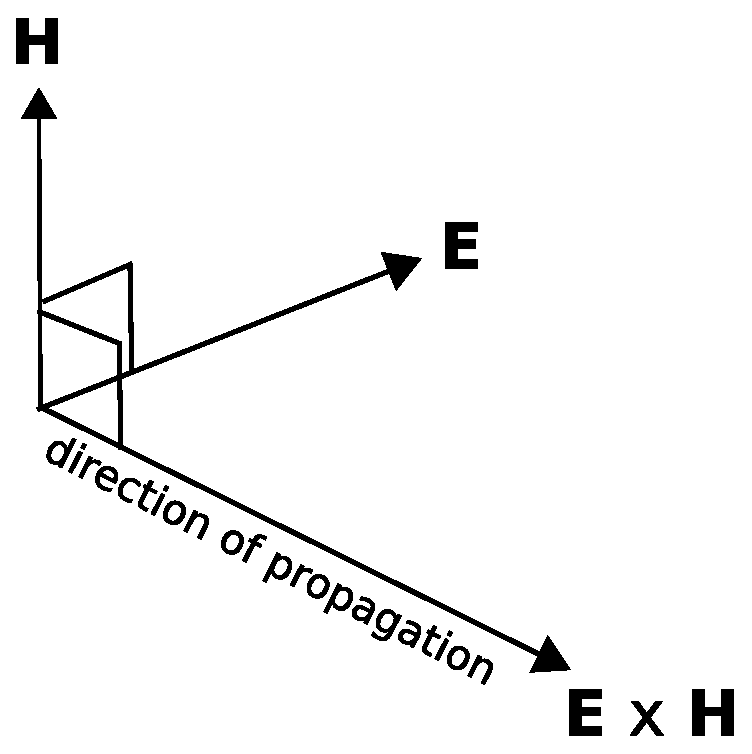
\includegraphics[width=2in]{modules/m0038_fEHk.eps}
% URL goes here
}}{A Cartesian plane with H, E, and E cross H axes. The H-axis points vertically. The E-axis and E cross H axes are perpendicular to the H-axis and each other. They are connected by the origin. The E cross H axis is labeled "direction of propagation".}
\end{center} 
%\centerline{\scriptsize 
%\copyright~\hyperref[m0039_Onde_electromagnetique_Credit]{E.\ Boutet} (Modified) 
%\href{https://creativecommons.org/licenses/by-sa/3.0/}{CC BY-SA 3.0} 
%} 
\caption{
\label{m0038_fEHk}
Relationship between the electric field direction, magnetic field direction, and direction of propagation.
}
\end{figure}
%

Now let us resolve the question of the factor relating $\widetilde{\bf E}$ and $\widetilde{\bf H}$.
The factor is now seen to be $\beta/\omega\mu$ in Equation~\ref{m0038_eHy}, which can be simplified as follows: 
%
\begin{equation}
\frac{\beta}{\omega\mu} = \frac{\omega\sqrt{\mu\epsilon}}{\omega\mu} = \frac{1}{\sqrt{\mu/\epsilon}}
\end{equation}
%
The factor $\sqrt{\mu/\epsilon}$ appearing above has units of $\Omega$ is known variously as the \emph{wave impedance} 
\index{wave impedance}
or the \emph{intrinsic impedance of the medium}.
Assigning this quantity the symbol ``$\eta$,'' we have:
%
\begin{equation}
\boxed{
\eta \triangleq \frac{\widetilde{E}_x}{\widetilde{H}_y} = \sqrt{\frac{\mu}{\epsilon}}
}
\label{m0038_eEta}
\end{equation}
%
%ORB HIGHLIGHT
\begin{mdframed}[backgroundcolor=yellow!20,nobreak=true] 
The ratio of the electric field intensity to the magnetic field intensity is the wave impedance $\eta$ (Equation~\ref{m0038_eEta}; units of $\Omega$).  
In lossless media, $\eta$ is determined by the ratio of permeability of the medium to the permittivity of the medium. 
\end{mdframed}
%
The wave impedance in free space, assigned the symbol $\eta_0$, is
%
\begin{equation}
\eta_0 \triangleq \sqrt{\frac{\mu_0}{\epsilon_0}} \cong 377~\Omega. 
\end{equation}

Wrapping up our solution, we find that if $\widetilde{\bf E}$ is as given by Equation~\ref{m0038_eEx}, then
%
\begin{equation}
\widetilde{\bf H} = \hat{\bf y}\frac{E_0}{\eta} e^{-j\beta z}
\end{equation}

%%% TODO Example: Change orientation of E, direction of propagation, what is new H; then reference m0039 (Plane Wave Relationship)

\index{waves!plane|)}
